\section{Verification purpose}

\textbf{Case ID:} \CaseID

This case verifies finite-duration firebrand generation when the source lifetime is not commensurate with the solver timestep. It compares timesteps shorter and longer than the residence time while holding the source, grid, wind, and transport distribution fixed.

The test exposes whole-step over-generation, truncation of the last active interval, and timestep-dependent deposition. Success requires both variants to recover the same integrated source count and downwind profile within tolerance.

\section{Mathematical formulation and numerical implementation}
Let a burning computational cell generate firebrands at the constant rate
$\mathrm{GR}$ from ignition time $t_{\mathrm{ign}}$ until
$t_{\mathrm{ign}}+t_{\mathrm{res}}$. The number generated during an ELMFIRE
step $[t,t+\Delta t]$ must use the overlap between that step and the active
source interval:
\[
  \Delta t_{\mathrm{active}}
  =\max\!\left(0,
    \min(t+\Delta t,t_{\mathrm{ign}}+t_{\mathrm{res}})
    -\max(t,t_{\mathrm{ign}})\right),
\]
\[
  \Delta N=\mathrm{GR}\,\Delta t_{\mathrm{active}}.
\]
This formulation handles the first and final partial steps and also handles a
single timestep that spans the entire residence time. Summing over all steps
must give
\[
  N_{\mathrm{total}}=\mathrm{GR}\,t_{\mathrm{res}}.
\]
The case sets $\mathrm{GR}=\Metric{generationratepcspers}$~pcs/s and
$t_{\mathrm{res}}=\Metric{residencetimes}$~s, so the expected total is
$\Metric{expectedtotal}$ firebrands.

\subsection{Implementation path and verification rationale}

The documented finite-duration source formulation identifies a timestep-integration
error when the solver step is comparable to or longer than the fireline residence
time~\cite{Qin2025}. In current ELMFIRE,
\texttt{READ\_SPOTTING} selects the \texttt{PER-AREA} source,
\texttt{SPOTTING} computes the active-cell emission, and the source timing
state maintained by \texttt{CALC\_SPOTTING\_DURATION} bounds that emission.
The accumulated Eulerian field is advanced by
\texttt{EMBER\_TRAJECTORY\_EULERIAN}. Comparing a fine step with a step
longer than the complete source lifetime directly tests whether partial-step
overlap, rather than the nominal solver step, controls the emitted amount.
The total-count metric detects temporal over- or under-integration; the profile
 additionally detects correct totals deposited in wrong cells.
Surface spread, ignition, consumption, and crosswind dispersion are disabled,
so those processes cannot compensate for a source-timing error. The test
verifies numerical accounting and the configured transport kernel, not the
physical realism of the prescribed lognormal distribution.

\section{Derivation of expected behavior}
Generated firebrands are distributed with a lognormal distance model using
$\mu=2.18$ and $\sigma=1.23$. The distribution is truncated at its 99th
percentile. ELMFIRE rounds that distance to an integer number $K$ of cells and
normalizes the retained probability:
\[
  P_i=\frac{F(i\Delta x)-F((i-1)\Delta x)}
             {F(K\Delta x)-F(10^{-6})},\qquad i=1,\ldots,K,
\]
where $F$ is the lognormal cumulative distribution. The analytical count in
cell $i$ is $N_i=100P_i$. The postprocessor reproduces this cell-integrated
reference and compares it directly with the final \texttt{ember\_flux} raster.

\section{Verification metrics and acceptance criteria}

The integrated reference count is
\(N_{\mathrm{ref}}=G_Rt_{\mathrm{res}}=10\times10=100\) particles. The analytical
spatial reference integrates the configured lognormal landing distribution over
each downwind cell, truncates it at the 99th percentile, and renormalizes the
cell probabilities to \(N_{\mathrm{ref}}\). The ignition row and physical columns
are read from each manifest; all halo cells and nodata values are excluded.

\subsection{Justification of metric quantification}

Both limits have a direct particle-count interpretation.  Since
\(N_{\mathrm{ref}}=100\), the integrated-error bound \(E_N\le0.005\) permits an
absolute imbalance of only 0.5 particle.  This is large enough for raster
roundoff and percentile-edge binning, but too small to hide a one-particle
source-duration error.  The normalized \(L_1\) bound of 0.01 permits at most
one particle's worth of total spatial redistribution after the analytical
lognormal probabilities have been integrated over the same cells.  Unlike a
signed error, this norm cannot conceal compensating upstream and downstream
errors.  Applying both conditions to the short- and long-timestep variants
separates conservation of the total from correct overlap-limited placement.
The exact variant count is required because the intended assertion concerns
both sides of the residence-time boundary.

\subsection{Predeclared acceptance contract}

Table~\ref{tab:acceptance-contract} summarizes the metrics fixed before
inspection of the calculated results. Numerical values and component statuses
are reported separately in Section~7.

\begin{table}[H]
\centering
\footnotesize
\caption{Predeclared verification metrics and acceptance criteria.}
\label{tab:acceptance-contract}
\begin{tabular}{@{}p{0.23\linewidth}p{0.47\linewidth}p{0.21\linewidth}@{}}
\toprule
Metric & Output, region, and aggregation & Acceptance criterion\\
\midrule
Output completeness & One final \path{ember_flux} raster with current manifest geometry for each timestep. & 2 of 2 variants usable \\
Integrated-count error & \(E_N=|\sum_{ij}N_{ij}-N_{\mathrm{ref}}|/N_{\mathrm{ref}}\), using the full valid output raster. & \(E_N\le0.005\) for each timestep \\
Profile normalized \(L_1\) error & \(E_{L_1}=\sum_k|N_k-N_{k,\mathrm{ref}}|/N_{\mathrm{ref}}\) on matched physical downwind cells. & \(E_{L_1}\le0.01\) for each timestep \\
Overall decision & Conjunction of output completeness and both errors for both timestep variants. & PASS only if every component passes \\
\bottomrule
\end{tabular}
\end{table}

\section{Simulation configuration and predicted outcome}

Figure~\ref{fig:input-configuration} records the prepared spatial inputs for \texttt{dt0p13}.
The postprocessor reads these panels from the variant-local GeoTIFF files, removes the
two-cell numerical buffer, and retains map coordinates in metres.  The left panel shows
the most informative fuel or structure layout available for the case; the right panel
shows the cells selected by the non-positive initial level-set field, making a localized
ignition or firebrand-emission source explicit.

\begin{figure}[H]
\centering

\includegraphics[width=0.98\textwidth,height=0.42\textheight,keepaspectratio]{../figures/input_configuration.pdf}
\caption{Whole-domain prepared input configuration for the representative variant.  The
physical domain is shown without the numerical halo; coordinates, configured wind values,
fuel or structure layout, and initial ignition/source geometry are identified in the panels.}
\label{fig:input-configuration}
\end{figure}

The preprocessor creates two variants with $\Delta t=0.13$~s and
$\Delta t=12.7$~s. Both use a 10~m grid and the same 500~m by 60~m physical
domain. This gives 50 by 6 usable cells and a 54 by 10 raster after two numerical buffer cells are added outside all four sides. A single
ignition is placed in the first usable column and the middle usable row.

The source is isolated with \texttt{NO\_SURFACE\_FIRE=.TRUE.}, so it does not
create additional burning cells. The current \texttt{PER-AREA} generation
model calculates
\[
  \mathrm{GR}_{\mathrm{pixel}}
  =\mathrm{EMBER\_GR}\,\Delta x\Delta y.
\]
Using \texttt{EMBER\_GR=0.1}~pcs/s/m$^2$ and a 100~m$^2$ cell gives the
required 10~pcs/s source. The fixed source duration is selected with
\texttt{USE\_PHYSICAL\_SPOTTING\_DURATION=.FALSE.} and
\texttt{TAU\_EMBERGEN=10}~s. Firebrand ignition, consumption, and crosswind
dispersion are disabled so that they cannot change the accumulated count.


Each variant must satisfy both conditions:
\begin{itemize}
  \item total-count relative error no greater than 0.5\%;
  \item profile $L_1$ relative error no greater than 1\%.
\end{itemize}
The overall case passes only if outputs exist and both timestep variants pass.
The two-cell buffers are excluded from profile extraction, while the total
count is checked over the complete raster to detect misplaced firebrands.

\section{Actual simulation results}

Figure~\ref{fig:domain-result} shows the representative accumulated firebrand density from \texttt{dt0p13}.
It is read from the actual ELMFIRE output named in the panel, masks nodata, and excludes
the two-cell numerical buffer.  Firebrand counts are normalized by the cell length and the represented 1-m cross-stream strip, giving units of pcs m$^{-2}$.

\begin{figure}[H]
\centering

\includegraphics[width=0.96\textwidth,height=0.50\textheight,keepaspectratio]{../figures/domain_result.pdf}
\caption{Whole-domain accumulated firebrand density from the representative completed ELMFIRE run.  This
domain-scale result supplements, rather than replaces, the higher-level verification
profiles, convergence plots, ensemble statistics, and calculated acceptance metrics below.}
\label{fig:domain-result}
\end{figure}


Overall status: \textbf{\Metric{status}}. Figure~\ref{fig:generation-duration}
first compares each actual ELMFIRE profile with the cell-integrated analytical
distribution. Agreement for the 12.7~s variant is the critical result because
that timestep exceeds the complete 10~s source duration.

\begin{figure}[H]
  \centering
  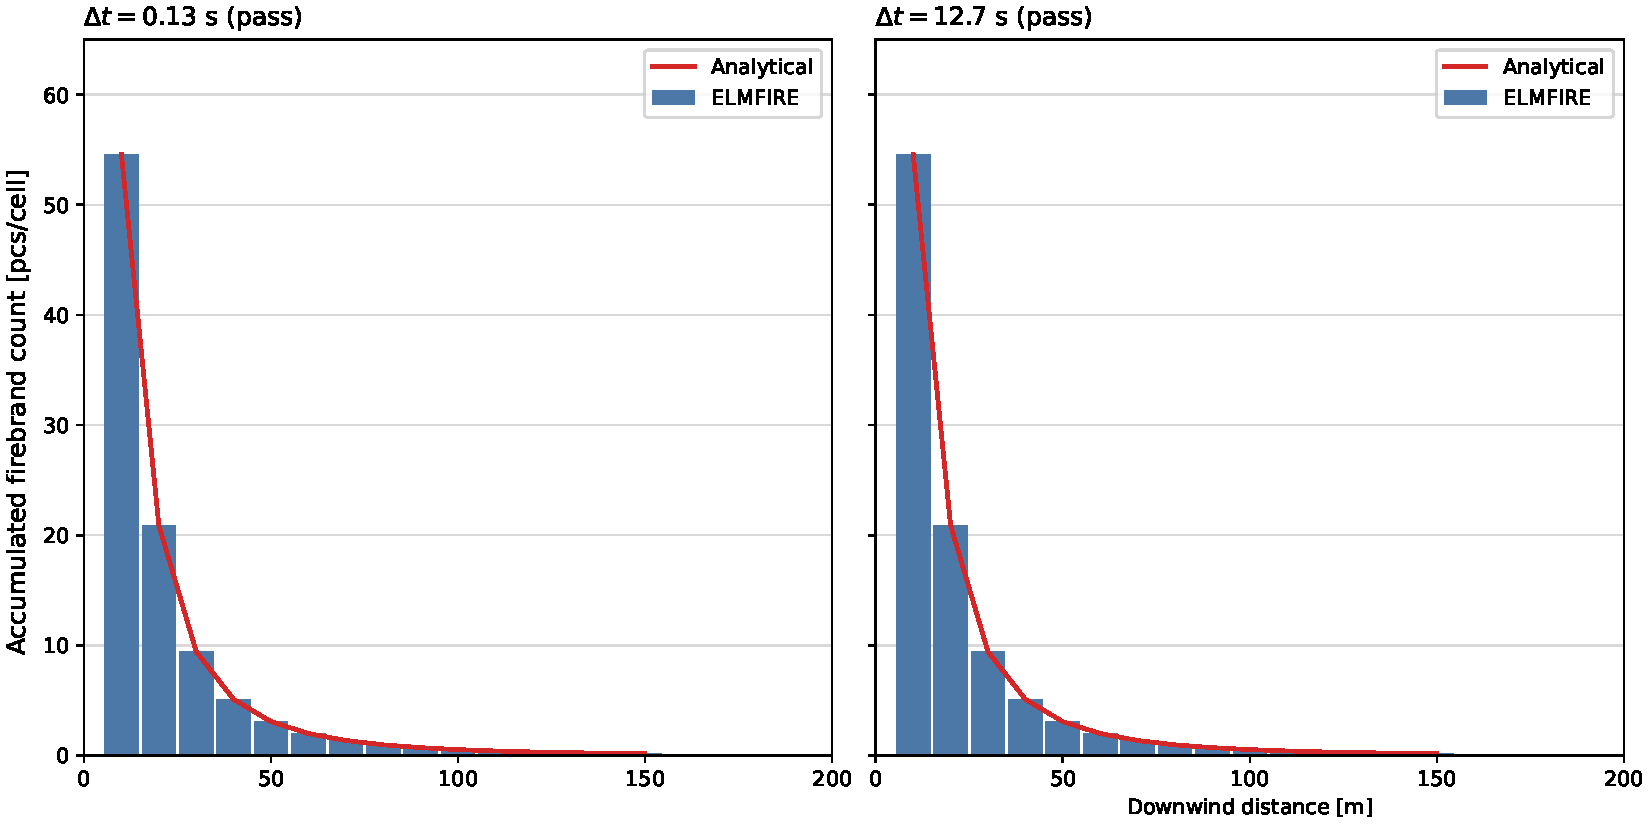
\includegraphics[width=\textwidth,height=0.62\textheight,keepaspectratio]{../figures/generation_residence_time.pdf}
  \caption{Accumulated firebrands per downwind cell for the 0.13 and 12.7~s
  timestep variants. Blue bars are ELMFIRE output and the red curve is the
  cell-integrated, truncated-lognormal reference for 100 generated firebrands.}
  \label{fig:generation-duration}
\end{figure}

% Figure~\ref{fig:generation-duration-errors} then isolates the two acceptance
% observables, making it clear whether any agreement in the spatial plot conceals
% a conservation error.

% \begin{figure}[H]
%   \centering
%   \includegraphics[width=0.78\textwidth,height=0.42\textheight,keepaspectratio]{../figures/generation_residence_time_errors.pdf}
%   \caption{Integrated-count and normalized profile errors for both timesteps,
%   with their separately predeclared acceptance limits.}
%   \label{fig:generation-duration-errors}
% \end{figure}

\section{Calculated metrics and verification decision}
\begin{table}[htbp]
\centering
\begin{tabular}{lrrr}
\toprule
Timestep & Observed total & Total relative error & Profile $L_1$ error \\
\midrule
0.13 s & \Metric{fineobservedtotal} & \Metric{finetotalrelativeerror} & \Metric{fineprofileloneerror} \\
12.7 s & \Metric{coarseobservedtotal} & \Metric{coarsetotalrelativeerror} & \Metric{coarseprofileloneerror} \\
\bottomrule
\end{tabular}
\caption{Firebrand-count and spatial-distribution errors for the two timestep variants.}
\end{table}

The overall decision is \textbf{\Metric{status}} and is taken directly from postprocessing.

\section{Technical interpretation}
Agreement of both totals and profiles across a timestep longer than the complete source duration demonstrates correct partial-step accounting; a discrepancy isolates temporal source integration or deposition indexing.

\section{Scope and limitations}
The generated variant namelists, raster dimensions, buffer width, source
location, rates, duration, and analytical parameters are recorded in
\texttt{../variants/manifest.json}. Per-variant raster filenames and numerical
errors are recorded in \texttt{../outputs/metrics.json}.

\begin{thebibliography}{9}
\bibitem{Qin2025}
Y. Qin, \emph{A Physics-Based Eulerian Framework for Modeling Firebrand
Showering in Regional-Scale Wildland and Wildland--Urban Interface Fire
Simulations}, Ph.D. dissertation, University of Maryland, College Park, 2025.
\end{thebibliography}
